% chktex-file 2% chktex-file 29
% chktex-file 13
\documentclass{report}
\usepackage{setspace}
\usepackage[a4paper, total={7in, 10in}]{geometry}
\usepackage[fleqn]{amsmath}
\usepackage{empheq}
\usepackage{amssymb}
\usepackage{amsthm}
\usepackage{gensymb}
\usepackage[fleqn]{cases}
\usepackage{multicol}
\usepackage{color}
\usepackage{stix}
\usepackage{chngcntr}
\usepackage{tikz}
\usepackage{enumitem}
\usepackage{pgfplots}
\usepackage{etoolbox}
\usepackage{tikz-3dplot}
\usepackage{tkz-euclide}
\usepackage{enumitem}

\def\nswe#1#2#3{#1\,$#2^\circ\,#3'$}
\graphicspath{ {./assets/} }
\usetikzlibrary{calc,matrix,arrows}
\usetikzlibrary{decorations.pathmorphing,patterns, calligraphy, perspective,backgrounds}

\counterwithout{equation}{chapter}
\setlength{\columnseprule}{1pt}
\setlength{\columnsep}{24pt}
\setcounter{chapter}{16}
\hfuzz=100pt

\newcommand{\pgfplotsdrawaxis}{\pgfplots@draw@axis}
\makeatother
\pgfplotsset{only axis on top/.style={axis on top=false, after end axis/.code={
                    \pgfplotsset{axis line style=opaque, ticklabel style=opaque, tick style={thick,opaque},
                        grid=none}\pgfplotsdrawaxis}}}

\newtheorem{theorem}{Theorem}

\begin{document}

\newcommand{\sol}[1]{

    \noindent \textbf{Sol.}
}
\newcommand{\prooff}[1]{

    \noindent \textbf{Proof.}
}
\newcommand\m[1]{\begin{pmatrix}#1\end{pmatrix}}
\newcommand\vm[1]{\begin{vmatrix}#1\end{vmatrix}}
\newenvironment{amatrix}[1]{%
    \left(\begin{array}{@{}*{#1}{c}|c@{}}
        }{%
    \end{array}\right)
}
\newenvironment{cequation}{
    \makeatletter
    \setbool{@fleqn}{false}
    \makeatother
    \begin{equation*}
        }{\end{equation*}}

\begin{titlepage}
    \raggedleft{}
    \rule{1pt}{\textheight}
    \hspace{0.02\textwidth}
    \parbox[b]{0.75\textwidth}{

    {\Huge\bfseries Solution Book of \\[0.5\baselineskip] Mathematic}\\[2\baselineskip]
    {\large\textit{Ssnior 2 Part I}}\\[4\baselineskip]
    {\Large\textsc{MELVIN CHIA}}

    \vspace{0.5\textheight}

    {\noindent Written on 9 October 2022}\\[\baselineskip]
    }

\end{titlepage}

\doublespacing{}
\tableofcontents
\singlespacing{}
\newpage

\begin{multicols}{2}
    \begin{enumerate}

        \item The diagram below shows a cuboid with volume of $300cm^3$. Given that $AD =
                  2DC$ and $DN = 9cm$. Find the angle formed by line $AM$ and plane $KLMN$.
              \begin{center}
                  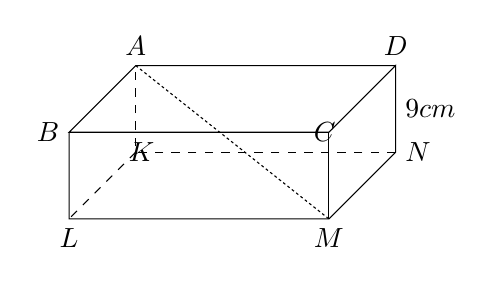
\begin{tikzpicture}[scale=1.1]
                      \draw (3,1,0) node [above] {$D$} --(0,1,0) node [above] {$A$} --(0,1,2) node [left] {$B$} --(3,1,2) node [above=6pt, left=-6pt] {$C$} --(3,1,0)--(3,0,0) node [right] {$N$} node [midway, right] {$9cm$}--(3,0,2)node [below] {$M$}--(0,0,2) node [below] {$L$} --(0,1,2);
                      \draw (3,1,2)--(3,0,2);
                      \draw[dashed](3,0,0)--(0,0,0) node [below=6pt, right=-6pt] {$K$}--(0,1,0);
                      \draw[dashed](0,0,0)--(0,0,2);
                      \draw[dash pattern=on 1pt off 1pt] (0, 1, 0) -- (3,0,2);
                  \end{tikzpicture}
              \end{center}

        \item The diagram below shows a cuboid. Given that $AB = 13cm$, $BC = 6cm$, $CG =
                  4cm$. M is a point on $AB$, $AM = 9cm$. Find:
              \begin{enumerate}
                  \item The angle formed by line $HM$ and plane $ABCG$.
                  \item The angle formed by line $HM$ and plane $HDAE$.
                  \item The angle formed by line $AG$ and plane $CDHG$.
              \end{enumerate}
              \begin{center}
                  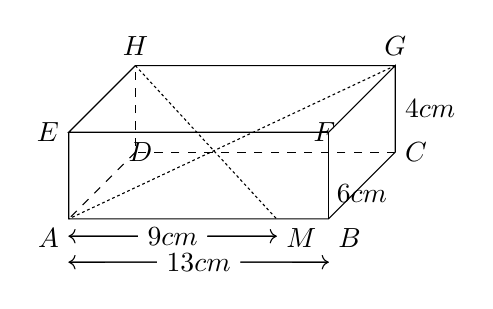
\begin{tikzpicture}[scale=1.1]
                      \draw (3,1,0) node [above] {$G$} --(0,1,0) node [above] {$H$} --(0,1,2) node [left] {$E$} --(3,1,2) node [above=6pt, left=-6pt] {$F$} --(3,1,0)--(3,0,0) node [right] {$C$} node [midway, right] {$4cm$}--(3,0,2)node [below right] {$B$} node [midway, right=16pt, below=-4pt] {$6cm$}--(0,0,2) node [below left] {$A$} --(0,1,2);
                      \draw (3,1,2)--(3,0,2);
                      \draw[dashed](3,0,0)--(0,0,0) node [below=6pt, right=-6pt] {$D$}--(0,1,0);
                      \draw[dashed](0,0,0)--(0,0,2);
                      \draw[dash pattern=on 1pt off 1pt] (0, 1, 0) -- (2.4,0,2) node [below right] {$M$};
                      \draw[dash pattern=on 1pt off 1pt] (3, 1, 0) -- (0, 0, 2);
                      \path (0, -0.2, 2) -- node (success) {$9cm$} (2.4, -0.2, 2);
                      \draw[->] (0, -0.2, 2) -- (success) -- (2.4, -0.2, 2);
                      \draw[->] (2.4, -0.2, 2) -- (success) -- (0, -0.2, 2);
                      \path (0, -0.5, 2) -- node (success) {$13cm$} (3, -0.5, 2);
                      \draw[->] (0, -0.5, 2) -- (success) -- (3, -0.5, 2);
                      \draw[->] (3, -0.5, 2) -- (success) -- (0, -0.5, 2);
                  \end{tikzpicture}
              \end{center}
        \item The diagram below shows a regular prism, its bases $ADS$ and $BCR$ are
              equiliteral triangles. Given that $AB = 16cm$, $BC = 7cm$, $SP = 5cm$. Find:
              \begin{enumerate}
                  \item The length of $BP$.
                  \item The angle formed by line $BP$ and plane $ABCD$.
              \end{enumerate}
              \begin{center}
                  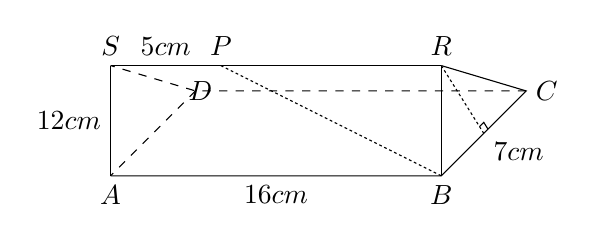
\begin{tikzpicture}[scale=1.4]
                      \draw (3,1,2) node [above] {$R$} --(0,1,2) node [above] {$S$};
                      \draw (3, 1, 2)--(3,0,0) node [right] {$C$} --(3,0,2)node [below] {$B$} node [midway, below right] {$7cm$} --(0,0,2) node [below] {$A$} node [midway, below] {$16cm$};
                      \draw (0,1,2) -- (0,0,2) node [midway, left] {$12cm$};
                      \draw (3,1,2) -- (3,0,2);
                      \draw[dashed](3,0,0)--(0,0,0) node [below=6pt, right=-6pt] {$D$}--(0,1,2);
                      \draw[dashed](0,0,0)--(0,0,2);
                      \draw[dash pattern=on 1pt off 1pt] (1, 1, 2) node [above] {$P$} -- (3,0,2);
                      \draw (0, 1, 2) -- (1, 1, 2) node [midway, above] {$5cm$};
                      \draw[dash pattern=on 1pt off 1pt] (3, 1, 2) -- (3, 0, 1);
                      \draw (3, 0.1, 1.1) -- (3, 0.1, 1) -- (3, 0, 0.9);
                  \end{tikzpicture}
              \end{center}
        \item The diagram below shows a roof, $HK$ is the ridge of the roof, its edges $HA$,
              $HD$, $KB$, $KC$ are euqal in length. Both of the planes $HAD$ and $KBC$ form a
              $44^o$ angle with plane $ABCD$. Given that $S$ and $T$ are the midpoints of
              $BC$ and $AD$ respectively. Find:
              \begin{enumerate}
                  \item The distance from line $HK$ to plane $ABCD$.
                  \item The length of $HK$.
                  \item The angle formed by line $HA$ and plane $ABCD$.
              \end{enumerate}
              \begin{center}
                  \includegraphics[scale=0.9]{roof}
              \end{center}
        \item The length, width and height of a hall are $20m$, $15m$, and $4m$ respectively.
              Find:
              \begin{enumerate}
                  \item The length of the diagonal of the hall.
                  \item The angle formed by the diagonal and the floor of the hall.
              \end{enumerate}
              \begin{center}
                  \includegraphics[scale=0.9]{hall}
              \end{center}
        \item In the diagram below, $ABCD$ represents a rectangular plank with length and
              width of $60cm$ and $36cm$ respectively, its base $BC$ is on the ground and the
              top of it lies on the wall. Assume that the distance between $BC$ and the
              corner of the wall is $12cm$, find the angle formed by the diagonal $BD$ of the
              plank and the ground.
              \begin{center}
                  \includegraphics[scale=0.9]{wall}
              \end{center}
    \end{enumerate}
\end{multicols}
\end{document}